\documentclass[11pt]{article}
\usepackage[letterpaper,margin=1in]{geometry}
\usepackage{amsmath,amssymb,amsthm,mathtools}
\usepackage{booktabs}
\usepackage{graphicx}
\usepackage{microtype}
\usepackage{enumitem}
\usepackage{hyperref}
\usepackage{url}
\usepackage{xcolor}
\usepackage{caption}
\usepackage{array}
\usepackage{siunitx}
\usepackage{fancyhdr}
\usepackage{lastpage}

\hypersetup{
  colorlinks=true,
  linkcolor=black,
  citecolor=black,
  urlcolor=blue,
  pdftitle={K-COS: Query-Adaptive Spectral Packetization for Certified Extreme-Tail Evaluation of Positive Gaussian Quadratic Forms},
  pdfauthor={Komorebi P.}
}

\pagestyle{fancy}
\setlength{\headheight}{14pt}
\fancyhf{}
\lhead{K-COS}
\rhead{Komorebi P.}
\cfoot{\thepage\ of \pageref{LastPage}}

\newtheorem{theorem}{Theorem}[section]
\newtheorem{proposition}[theorem]{Proposition}
\newtheorem{lemma}[theorem]{Lemma}
\newtheorem{corollary}[theorem]{Corollary}
\theoremstyle{definition}
\newtheorem{definition}[theorem]{Definition}
\newtheorem{remark}[theorem]{Remark}

\DeclareMathOperator{\E}{\mathbb E}
\DeclareMathOperator{\Var}{Var}
\newcommand{\R}{\mathbb R}
\newcommand{\C}{\mathbb C}
\newcommand{\Pp}{\mathbb P}
\newcommand{\eps}{\varepsilon}
\newcommand{\ii}{\mathrm{i}}
\newcommand{\phit}{\phi_{\theta}}

\title{\textbf{K-COS: Query-Adaptive Spectral Packetization for Certified Extreme-Tail Evaluation of Positive Gaussian Quadratic Forms}}
\author{Komorebi P.}
\date{September 2026}

\begin{document}
\maketitle

\begin{abstract}
We study numerical evaluation of upper-tail probabilities for positive Gaussian quadratic forms
\[
Q=\sum_{j=1}^{r}\lambda_j Z_j^2,
\qquad \lambda_j>0,
\qquad Z_j\stackrel{\mathrm{iid}}{\sim}N(0,1),
\]
with particular attention to small probabilities and repeated evaluations from large kernel spectra. The proposed method, called K-COS, combines three ideas: exponential tilting centered at the requested threshold, a query-dependent compression of the spectrum into centered moment packets, and a Fourier-cosine inversion whose three main analytic approximation errors are tracked separately. For a spectral packet with center $\mu$ and deviations $\delta_j$, the cumulant generating function admits a local expansion in centered power sums with an explicit geometric remainder bound on the complex frequency grid used by COS. We derive a finite-grid propagation bound from the log-transform error to the tail probability, a positive-support bound controlling upper truncation and cosine periodization, and an omitted-mode bound based on the monotone logarithmic decay rate of the tilted characteristic function. These terms yield a computable analytic relative-error certificate. A conditional refinement theorem shows that, for every fixed positive spectrum and upper-tail query, all three analytic error terms can be driven below any prescribed tolerance by finitely many packet splits, support expansions, and mode refinements. Prototype experiments on exactly solvable chi-square laws and genotype-derived SKAT-like spectra support the derivation. At a requested relative tolerance of $10^{-8}$, twelve extreme-tail experiments returned valid analytic certificates, with worst observed relative error $6.15\times10^{-11}$ and largest certified bound $7.92\times10^{-9}$. The current work does not yet provide directed-rounding control of floating-point transcendental operations and has not yet been benchmarked against Davies' algorithm or Imhof inversion; those comparisons are required before making a production-level superiority claim.
\end{abstract}

\noindent\textbf{Status.} This is a research formalization of a tested prototype. Theorems below concern the stated mathematical model and analytic error decomposition. Novelty claims are deliberately provisional pending a deeper prior-art audit and direct comparison against established generalized-chi-square solvers.

\section{Problem and motivation}

Positive Gaussian quadratic forms appear in variance-component tests, kernel methods, random-effects models, and many other settings. Their null laws reduce to weighted sums of independent chi-square variables. Classical numerical approaches include characteristic-function inversion due to Imhof and Davies, series methods in positive-weight cases, saddlepoint approximations, and more recent generalized-chi-square algorithms. In genetic association testing, the sequence kernel association test (SKAT) is a prominent example in which the score statistic has a mixture-of-chi-square null distribution \cite{Wu2011}.

The Fourier-cosine (COS) method introduced by Fang and Oosterlee recovers expectations and distributional quantities from characteristic functions using cosine coefficients \cite{FangOosterlee2008}. Subsequent work has sharpened the choice of truncation range and number of modes \cite{Junike2024}, while the damped COS framework makes exponential reweighting explicit in a general characteristic-function setting \cite{JunikeStier2025}. Thus neither exponential damping nor COS inversion is claimed as new here.

The question addressed in this paper is narrower:
\begin{quote}
Can the \emph{spectrum itself} be compiled into a smaller, query-specific representation before COS inversion, while retaining an explicit approximation certificate for the requested tail probability?
\end{quote}

The proposed answer is a centered spectral packet representation. Instead of evaluating every eigenvalue at every complex COS frequency, nearby eigenvalues are grouped around packet centers and represented through centered moments. The packetization is refined according to the actual tilted complex grid associated with the requested threshold $q$ and tolerance $\eps$.

\section{Quadratic-form transform and saddlepoint tilt}

Let
\begin{equation}
Q=\sum_{j=1}^{r}\lambda_j Z_j^2,
\qquad \lambda_j>0.
\label{eq:Q}
\end{equation}
The moment generating function exists for
\[
\Re s < \frac{1}{2\lambda_{\max}},
\qquad
\lambda_{\max}=\max_j\lambda_j,
\]
and its cumulant generating function is
\begin{equation}
\kappa(s)=\log \E e^{sQ}
=-\frac12\sum_{j=1}^{r}\log(1-2s\lambda_j).
\label{eq:cgf}
\end{equation}
For real $\theta<1/(2\lambda_{\max})$,
\begin{equation}
\kappa^{(m)}(\theta)
=2^{m-1}(m-1)!\sum_{j=1}^{r}
\frac{\lambda_j^m}{(1-2\theta\lambda_j)^m},
\qquad m\ge1.
\label{eq:derivatives}
\end{equation}
At $\theta=0$, this recovers the standard cumulant identity
\[
\operatorname{cum}_m(Q)=2^{m-1}(m-1)!\sum_j\lambda_j^m.
\]

\begin{theorem}[Unique upper-tail saddlepoint]
\label{thm:saddle}
If $q>\E Q=\sum_j\lambda_j$, there exists a unique
\[
\theta_*=\theta(q)\in\left(0,\frac{1}{2\lambda_{\max}}\right)
\]
satisfying
\begin{equation}
\kappa'(\theta_*)=q.
\label{eq:saddle}
\end{equation}
\end{theorem}

\begin{proof}
By \eqref{eq:derivatives},
\[
\kappa'(\theta)=\sum_j\frac{\lambda_j}{1-2\theta\lambda_j}
\]
is continuous and strictly increasing on the stated interval. It equals $\E Q$ at $\theta=0$ and diverges as $\theta\uparrow1/(2\lambda_{\max})$. The intermediate value theorem and strict monotonicity give existence and uniqueness.
\end{proof}

Define the exponentially tilted law by
\begin{equation}
f_{\theta}(x)=e^{\theta x-\kappa(\theta)}f(x).
\label{eq:tilt-density}
\end{equation}
Its characteristic function is
\begin{equation}
\phi_{\theta}(t)
=\exp\{\kappa(\theta+\ii t)-\kappa(\theta)\},
\label{eq:tilt-cf}
\end{equation}
and $\E_{\theta}Q=\kappa'(\theta)$. Therefore the choice \eqref{eq:saddle} moves the query $q$ to the mean of the tilted law.

For any $\theta>0$ in the transform domain,
\begin{equation}
\Pp(Q\ge q)
=e^{\kappa(\theta)-\theta q}
\E_{\theta}\!\left[e^{-\theta(Q-q)}\mathbf 1_{\{Q\ge q\}}\right].
\label{eq:tilt-tail}
\end{equation}
This identity is classical exponential tilting; K-COS uses it to avoid subtracting a CDF value numerically close to one.

\section{Centered spectral packets}

Let a packet $P\subset\{1,\ldots,r\}$ contain $n_P$ eigenvalues. Define its center
\[
\mu_P=\frac{1}{n_P}\sum_{j\in P}\lambda_j,
\qquad
\delta_j=\lambda_j-\mu_P,
\]
and centered moments
\begin{equation}
M_{P,m}=\sum_{j\in P}\delta_j^m,
\qquad m\ge0.
\label{eq:centeredmoments}
\end{equation}
Thus $M_{P,0}=n_P$ and $M_{P,1}=0$.

\begin{theorem}[Centered packet expansion]
\label{thm:packet}
Fix $s\in\C$ such that $1-2s\mu_P\ne0$, and define
\begin{equation}
\alpha_P(s)=\frac{2s}{1-2s\mu_P},
\qquad
\rho_P(s)=|\alpha_P(s)|\max_{j\in P}|\delta_j|.
\label{eq:alpha-rho}
\end{equation}
If $\rho_P(s)<1$, then the packet contribution to \eqref{eq:cgf} is
\begin{align}
\kappa_P(s)
&=-\frac{n_P}{2}\log(1-2s\mu_P)
+\frac12\sum_{m=1}^{p}
\frac{\alpha_P(s)^m}{m}M_{P,m}
+R_{P,p}(s),
\label{eq:packet-expansion}
\end{align}
where
\begin{equation}
|R_{P,p}(s)|
\le
\frac{n_P}{2}
\frac{\rho_P(s)^{p+1}}{(p+1)(1-\rho_P(s))}.
\label{eq:packet-remainder}
\end{equation}
\end{theorem}

\begin{proof}
For $j\in P$,
\[
1-2s\lambda_j
=(1-2s\mu_P)(1-\alpha_P(s)\delta_j).
\]
Hence
\[
-\frac12\log(1-2s\lambda_j)
=-\frac12\log(1-2s\mu_P)
-\frac12\log(1-\alpha_P\delta_j).
\]
When $|\alpha_P\delta_j|<1$,
\[
-\log(1-z)=\sum_{m\ge1}\frac{z^m}{m}.
\]
Summing over $j\in P$ gives \eqref{eq:packet-expansion}. The remainder satisfies
\[
\left|\sum_{m\ge p+1}\frac{z^m}{m}\right|
\le
\sum_{m\ge p+1}\frac{|z|^m}{p+1}
=\frac{|z|^{p+1}}{(p+1)(1-|z|)}.
\]
Using $|z|\le\rho_P(s)$ and summing $n_P$ terms yields \eqref{eq:packet-remainder}.
\end{proof}

\begin{remark}[What is compressed]
A packet of $n_P$ eigenvalues is replaced by its center and $p$ centered moments. Large spectral spikes may be retained exactly. If the representation contains $s$ exact eigenvalues and $R$ packets of order $p$, evaluation of the CGF on $N$ frequencies costs $O(N(s+Rp))$ arithmetic operations after compilation, instead of $O(Nr)$ direct eigenvalue-transform evaluations.
\end{remark}

\begin{remark}[Query dependence]
The relevant packet condition is not merely geometric closeness of eigenvalues. It is the complex-grid quantity $\rho_P(\theta_*+\ii u_k)$. Thus a partition suitable for one tail query or one COS grid need not be suitable for another.
\end{remark}

\section{Tilted COS tail functional}

Because $Q\ge0$, K-COS uses the interval $[0,b]$. Let
\[
u_k=\frac{k\pi}{b},
\qquad k=0,1,\ldots,
\]
and define the exponentially weighted cosine integrals
\begin{equation}
J_k(q,b,\theta)
=\int_q^b e^{-\theta(x-q)}\cos(u_kx)\,dx.
\label{eq:J-def}
\end{equation}
They admit the closed form
\begin{equation}
J_k
=\Re\left[
 e^{\ii u_k q}
 \frac{1-e^{(-\theta+\ii u_k)(b-q)}}{\theta-\ii u_k}
\right].
\label{eq:J-formula}
\end{equation}
The prime on a cosine sum denotes half weight for $k=0$.

If the exact tilted characteristic function is used, the $N$-mode finite-window expression is
\begin{equation}
T_{N,b}
=\frac{2}{b}\sum_{k=0}^{N-1}{}'
J_k\,
\Re\left[e^{\kappa(\theta+\ii u_k)-\theta q}\right].
\label{eq:tail-cos}
\end{equation}
The cancellation of $\kappa(\theta)$ in \eqref{eq:tail-cos} is useful numerically: the likelihood-ratio prefactor from \eqref{eq:tilt-tail} and the normalization in \eqref{eq:tilt-cf} do not need to be formed separately inside each mode.

\section{Propagation of packet error}

Let $\widehat\kappa(s_k)$ be the packet approximation at
\[
s_k=\theta+\ii u_k,
\]
and suppose
\begin{equation}
|\widehat\kappa(s_k)-\kappa(s_k)|\le B_k.
\label{eq:Bk}
\end{equation}
For disjoint packets, $B_k$ can be chosen as the sum of the packet bounds \eqref{eq:packet-remainder}.

\begin{theorem}[Finite-grid packet-to-tail bound]
\label{thm:packet-tail}
Let $\widehat T_{N,b}$ be obtained from \eqref{eq:tail-cos} by replacing $\kappa(s_k)$ by $\widehat\kappa(s_k)$. Then
\begin{equation}
|\widehat T_{N,b}-T_{N,b}|
\le \eps_{\mathrm{pkt}},
\label{eq:packet-tail-bound}
\end{equation}
where
\begin{equation}
\eps_{\mathrm{pkt}}
=
\frac{2}{b}
 e^{\kappa(\theta)-\theta q}
\sum_{k=0}^{N-1}{}'
|J_k|\bigl(e^{B_k}-1\bigr).
\label{eq:eps-pkt}
\end{equation}
\end{theorem}

\begin{proof}
Write $\Delta_k=\widehat\kappa(s_k)-\kappa(s_k)$. Then
\[
|e^{\widehat\kappa(s_k)-\theta q}-e^{\kappa(s_k)-\theta q}|
\le
|e^{\kappa(s_k)-\theta q}|\,(e^{|\Delta_k|}-1).
\]
Moreover
\[
\Re\kappa(\theta+\ii u_k)-\kappa(\theta)
=\log|\phi_{\theta}(u_k)|\le0,
\]
so
\[
|e^{\kappa(s_k)-\theta q}|
\le e^{\kappa(\theta)-\theta q}.
\]
Substitute this into the finite cosine sum and apply the triangle inequality.
\end{proof}

\section{Positive support, truncation, and cosine periodization}

Using full characteristic-function coefficients on $[0,b]$ reconstructs the even $2b$-periodization of the tilted density rather than the strictly truncated density. For a nonnegative density supported on $[0,\infty)$, the total mass folded back into $[0,b]$ equals the tilted mass above $b$. This gives a clean error control for the positive quadratic-form setting.

\begin{proposition}[Support and periodization bound]
\label{prop:support}
Assume the tilted density is integrable and its cosine representation is valid in the sense required to integrate the resulting series against the bounded weight in \eqref{eq:tilt-tail}. Let
\[
\tau_{\theta}(b)=\Pp_{\theta}(Q>b).
\]
Then the combined error from (i) replacing the tilted density on $[0,b]$ by its full-coefficient cosine periodization and (ii) omitting the original integral over $(b,\infty)$ is bounded by
\begin{equation}
\eps_{\mathrm{sup}}
\le
e^{\kappa(\theta)-\theta q}\,
\tau_{\theta}(b)
\left(1+e^{-\theta(b-q)}\right).
\label{eq:eps-support}
\end{equation}
\end{proposition}

\begin{proof}
The alias density induced on $[0,b]$ by even $2b$-periodization is nonnegative and has total mass $\tau_{\theta}(b)$. On $[q,b]$, the weight $e^{-\theta(x-q)}$ is at most one, so its contribution to the weighted functional is at most $\tau_{\theta}(b)$. For the omitted original tail, $x\ge b$ implies
\[
e^{-\theta(x-q)}\le e^{-\theta(b-q)},
\]
so that term is at most $e^{-\theta(b-q)}\tau_{\theta}(b)$. Multiplication by the likelihood-ratio prefactor in \eqref{eq:tilt-tail} gives \eqref{eq:eps-support}.
\end{proof}

The tilted tail probability itself can be bounded by Chernoff's inequality. For $\eta>\theta$ inside the transform domain,
\begin{equation}
\tau_{\theta}(b)
\le
\exp\left\{
\kappa(\eta)-\kappa(\theta)-(\eta-\theta)b
\right\}.
\label{eq:tilted-chernoff}
\end{equation}
When $b>\kappa'(\theta)$, the minimizing $\eta$ is the unique solution of
\begin{equation}
\kappa'(\eta)=b.
\label{eq:eta}
\end{equation}
For the saddlepoint tilt, $\kappa'(\theta_*)=q<b$, so such an $\eta$ exists.

\section{A specialized omitted-mode bound}

The tilted characteristic function has an especially transparent modulus.

\begin{lemma}[Tilted characteristic-function modulus]
\label{lem:modulus}
Define
\begin{equation}
a_j=\frac{2\lambda_j}{1-2\theta\lambda_j}>0.
\label{eq:aj}
\end{equation}
Then
\begin{equation}
|\phi_{\theta}(t)|
=\prod_{j=1}^{r}\left(1+(a_jt)^2\right)^{-1/4}.
\label{eq:phi-modulus}
\end{equation}
Define the logarithmic decay rate
\begin{equation}
\beta(t)
=-\frac{d\log|\phi_{\theta}(t)|}{d\log t}
=\frac12\sum_{j=1}^{r}
\frac{(a_jt)^2}{1+(a_jt)^2}.
\label{eq:beta}
\end{equation}
Then $\beta(t)$ is nondecreasing for $t\ge0$.
\end{lemma}

\begin{proof}
Taking the modulus of each factor in \eqref{eq:tilt-cf} gives \eqref{eq:phi-modulus}. Differentiating its logarithm gives \eqref{eq:beta}. Each summand $x/(1+x)$ with $x=(a_jt)^2$ is nondecreasing in $t$.
\end{proof}

\begin{corollary}[Power envelope from one frequency]
\label{cor:power-envelope}
For $t\ge t_0>0$,
\begin{equation}
|\phi_{\theta}(t)|
\le
|\phi_{\theta}(t_0)|
\left(\frac{t}{t_0}\right)^{-\beta(t_0)}.
\label{eq:power-envelope}
\end{equation}
\end{corollary}

\begin{proof}
By Lemma \ref{lem:modulus},
\[
\frac{d\log|\phi_{\theta}(t)|}{d\log t}=-\beta(t)\le-\beta(t_0)
\]
for $t\ge t_0$. Integrating from $t_0$ to $t$ proves the claim.
\end{proof}

For $k\ge1$, the exact integral \eqref{eq:J-formula} implies
\begin{equation}
|J_k|
\le \frac{2}{u_k}.
\label{eq:J-bound}
\end{equation}

\begin{theorem}[Omitted COS-mode certificate]
\label{thm:cos-tail}
Let $u_N=N\pi/b$ and $\beta_N=\beta(u_N)$. If $\beta_N>0$, then the contribution of all exact tilted-COS modes $k\ge N$ to the weighted tail functional is bounded by
\begin{equation}
\eps_{\mathrm{COS}}
\le
 e^{\kappa(\theta)-\theta q}
\frac{4|\phi_{\theta}(u_N)|}{\pi}
\left(\frac1N+\frac1{\beta_N}\right).
\label{eq:eps-cos}
\end{equation}
\end{theorem}

\begin{proof}
Using the cosine coefficient magnitude $2|\phi_{\theta}(u_k)|/b$ and \eqref{eq:J-bound}, the omitted series is at most
\[
e^{\kappa(\theta)-\theta q}
\frac{4}{\pi}
\sum_{k=N}^{\infty}\frac{|\phi_{\theta}(u_k)|}{k}.
\]
By Corollary \ref{cor:power-envelope},
\[
|\phi_{\theta}(u_k)|
\le
|\phi_{\theta}(u_N)|\left(\frac{k}{N}\right)^{-\beta_N}.
\]
Therefore
\[
\sum_{k=N}^{\infty}\frac{|\phi_{\theta}(u_k)|}{k}
\le
|\phi_{\theta}(u_N)|N^{\beta_N}
\sum_{k=N}^{\infty}k^{-\beta_N-1}.
\]
Finally,
\[
\sum_{k=N}^{\infty}k^{-\beta_N-1}
\le N^{-\beta_N-1}+\int_N^{\infty}x^{-\beta_N-1}\,dx
=N^{-\beta_N-1}+\frac{N^{-\beta_N}}{\beta_N},
\]
which yields \eqref{eq:eps-cos}.
\end{proof}

\section{Combined analytic certificate}

\begin{theorem}[K-COS analytic error certificate]
\label{thm:combined}
Let $p=\Pp(Q\ge q)$, and let $\widehat p$ be the finite K-COS approximation formed with
\begin{enumerate}[label=(\roman*)]
\item an upper interval endpoint $b>q$,
\item $N$ cosine modes,
\item a packet approximation satisfying \eqref{eq:Bk} on the finite grid.
\end{enumerate}
Under the hypotheses of Proposition \ref{prop:support},
\begin{equation}
|p-\widehat p|
\le
\eps_{\mathrm{an}}
:=\eps_{\mathrm{pkt}}+\eps_{\mathrm{sup}}+\eps_{\mathrm{COS}}.
\label{eq:combined}
\end{equation}
If $\eps_{\mathrm{an}}<|\widehat p|$, then
\begin{equation}
\frac{|p-\widehat p|}{|p|}
\le
\frac{\eps_{\mathrm{an}}}
{|\widehat p|-\eps_{\mathrm{an}}}.
\label{eq:relative-certificate}
\end{equation}
\end{theorem}

\begin{proof}
Decompose the error into packet error on the retained grid, support and periodization error, and the exact omitted cosine series. The first is bounded by Theorem \ref{thm:packet-tail}, the second by Proposition \ref{prop:support}, and the third by Theorem \ref{thm:cos-tail}. This proves \eqref{eq:combined}. Also
\[
|p|\ge |\widehat p|-|p-\widehat p|
\ge |\widehat p|-\eps_{\mathrm{an}},
\]
which gives \eqref{eq:relative-certificate}.
\end{proof}

\begin{remark}[Certificate boundary]
Theorem \ref{thm:combined} is an \emph{analytic approximation certificate}. It does not enclose IEEE floating-point rounding in complex logarithms, exponentials, root finding, or summation. A machine-level certificate would require directed rounding, interval arithmetic, or a comparable validated-numerics layer.
\end{remark}

\section{Finite refinability}

The combined error terms correspond to three distinct obstructions. Packet error is reduced by splitting spectral packets or raising packet order; support error is reduced by increasing $b$; cosine-series error is reduced by increasing $N$.

\begin{proposition}[Existence of a finite analytic refinement]
\label{prop:finite-refinement}
Fix a finite positive spectrum $\{\lambda_j\}_{j=1}^{r}$, an upper-tail query $q>\E Q$, and $\eps>0$. There exist a finite interval endpoint $b>q$, a finite number of cosine modes $N$, and a finite packet partition (allowing singleton packets) for which the analytic error bound in \eqref{eq:combined} is below $\eps$.
\end{proposition}

\begin{proof}
First choose $b$ sufficiently large that \eqref{eq:eps-support} is below $\eps/3$. This is possible because the tilted law has a moment generating function in a nontrivial right neighborhood of zero and hence its Chernoff bound tends to zero exponentially as $b\to\infty$. Hold this $b$ fixed. By \eqref{eq:phi-modulus}, $|\phi_{\theta}(t)|\to0$ polynomially as $t\to\infty$, while $\beta(t)\to r/2>0$. Therefore \eqref{eq:eps-cos} tends to zero as $N\to\infty$, so a finite $N$ makes it below $\eps/3$. Finally, split every packet to singletons if necessary. A singleton has $\delta_j=0$, so its packet remainder is exactly zero. Hence a finite partition makes $\eps_{\mathrm{pkt}}<\eps/3$. Summing the three terms proves the claim.
\end{proof}

\begin{remark}
Proposition \ref{prop:finite-refinement} proves existence of a finite representation meeting any analytic tolerance. It does not by itself prove that every possible greedy refinement schedule terminates optimally. The prototype planner refines the largest currently certified obstruction and is evaluated empirically below.
\end{remark}

\section{Adaptive K-COS algorithm}

The prototype accepts $(\lambda_1,\ldots,\lambda_r,q,\tau)$, where $\tau$ is a requested relative tolerance.

\begin{enumerate}[leftmargin=2em]
\item Solve $\kappa'(\theta_*)=q$.
\item Initialize an upper interval $b=q+L\sqrt{\kappa''(\theta_*)+\sqrt{\kappa^{(4)}(\theta_*)}}$ and a mode count $N$.
\item Retain the largest spectral spikes exactly and place the remaining sorted eigenvalues into coarse packets.
\item Evaluate $\rho_P(\theta_*+\ii u_k)$ and the packet remainder bound on the actual COS grid. Split packets until the propagated packet contribution is within its budget.
\item Evaluate the support/alias certificate from \eqref{eq:eps-support}--\eqref{eq:eta}.
\item Evaluate the omitted-mode certificate \eqref{eq:eps-cos}.
\item If the combined relative certificate exceeds $\tau$, refine whichever analytic error source dominates: split packets, increase $b$, or increase $N$.
\item Return the tail probability, the compiled spectral passport, and the error ledger.
\end{enumerate}

The resulting object is query dependent. Schematically,
\begin{equation}
(\Lambda,q,\tau)
\longmapsto
\mathcal P_{\Lambda,q,\tau}
\longmapsto
(\widehat p,\text{certificate}),
\label{eq:compiler-map}
\end{equation}
where $\mathcal P_{\Lambda,q,\tau}$ stores exact spikes, packet centers, centered moments, packet radii, and the selected COS parameters.

\section{Numerical experiments}

\subsection{Exactly solvable chi-square stress test}

To isolate the effect of exponential tilting, we first used
\[
Q=0.02\chi^2_{80},
\]
whose survival probabilities are available directly from the chi-square distribution. Table \ref{tab:chi} compares a global COS calculation with query-centered tilted COS.

\begin{table}[htbp]
\centering
\caption{Relative error in an exactly solvable chi-square family.}
\label{tab:chi}
\begin{tabular}{rrrr}
\toprule
True tail $p$ & $N$ & Global COS rel. error & Tilted COS rel. error\\
\midrule
$10^{-6}$  & 64  & $3.56\times10^{-8}$ & $2.71\times10^{-14}$\\
$10^{-10}$ & 64  & $1.64\times10^{-4}$ & $6.59\times10^{-15}$\\
$10^{-10}$ & 128 & $2.03\times10^{-6}$ & $9.05\times10^{-15}$\\
$10^{-14}$ & 64  & $1.43$              & $3.53\times10^{-14}$\\
$10^{-14}$ & 128 & $6.15\times10^{-2}$ & $3.87\times10^{-14}$\\
\bottomrule
\end{tabular}
\end{table}

The test demonstrates the numerical motivation for tilting: evaluating a small tail directly under the shifted law is substantially more stable than reconstructing a global CDF and subtracting from one. This observation is not a novelty claim for exponential tilting itself.

\subsection{Genotype-derived spectra}

The second experiment used the existing Komorebi SKAT benchmark generator. Synthetic genotype matrices were centered and scaled, residualized against three covariates, weighted by $(1-\mathrm{MAF})^{24}$, and converted to the positive quadratic-form spectrum
\[
\lambda=\tfrac12\operatorname{eig}(AA^{\mathsf T}).
\]
Three independent $n=400$, $m=1200$ genotype sets yielded numerical rank $397$. Four upper-tail queries per spectrum were generated by choosing saddlepoint locations at fractions $0.70,0.80,0.85,0.90$ of the transform singularity. The comparison reference used exact-spectrum tilted COS with $N=2048$ and a large support parameter $L=20$. The adaptive method was asked for a relative analytic tolerance of $10^{-8}$.

Across the twelve queries:
\begin{itemize}
\item every requested $10^{-8}$ analytic certificate passed;
\item the worst observed relative error was $6.148608\times10^{-11}$;
\item the largest returned certified relative bound was $7.917203\times10^{-9}$;
\item the planner selected $N\in\{64,128\}$, $L\in\{10,11,12,13\}$, and 11--16 packets.
\end{itemize}

Figure \ref{fig:coverage} plots the observed errors against the returned analytic bounds. Every point lies above the equality line because the vertical coordinate is the bound.

\begin{figure}[htbp]
\centering
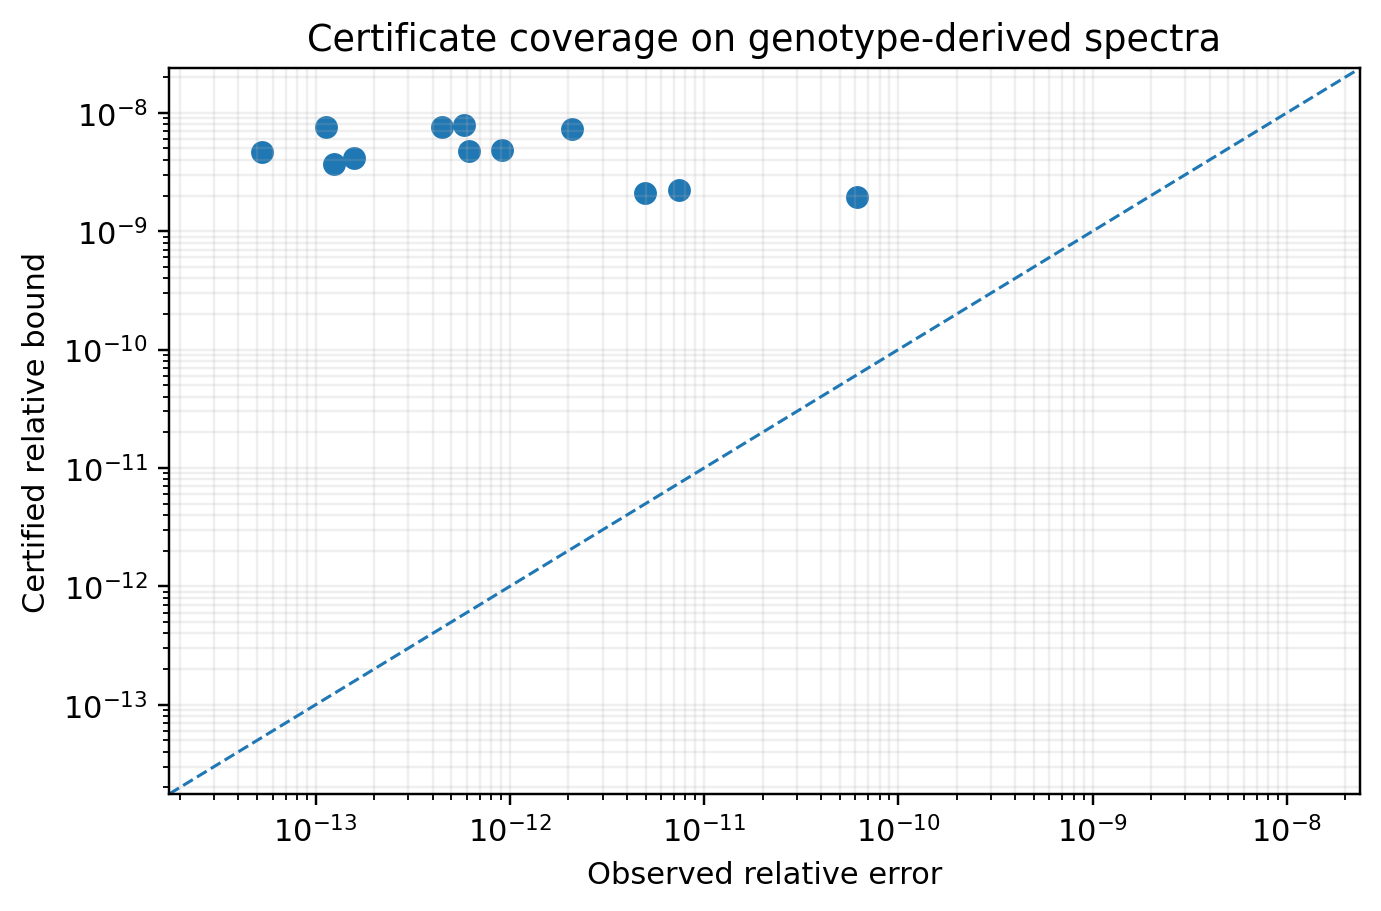
\includegraphics[width=0.78\linewidth]{figures/certificate_coverage.png}
\caption{Observed relative error versus the analytic certificate on twelve genotype-derived tail queries. The dashed line is equality.}
\label{fig:coverage}
\end{figure}

\subsection{Tolerance ladder}

At a reference tail probability near $8.99\times10^{-15}$, the same engine was requested to meet three tolerances. Table \ref{tab:ladder} shows how the representation refined automatically.

\begin{table}[htbp]
\centering
\caption{Adaptive refinement at an extreme-tail query.}
\label{tab:ladder}
\begin{tabular}{rrrrrr}
\toprule
Requested $\tau$ & $N$ & $L$ & Packets & Certified bound & Observed error\\
\midrule
$10^{-6}$  & 128 & 10 & 10 & $3.56\times10^{-7}$  & $3.63\times10^{-12}$\\
$10^{-8}$  & 128 & 12 & 15 & $4.87\times10^{-9}$  & $9.14\times10^{-13}$\\
$10^{-10}$ & 256 & 14 & 24 & $8.21\times10^{-11}$ & $5.65\times10^{-14}$\\
\bottomrule
\end{tabular}
\end{table}

\begin{figure}[htbp]
\centering
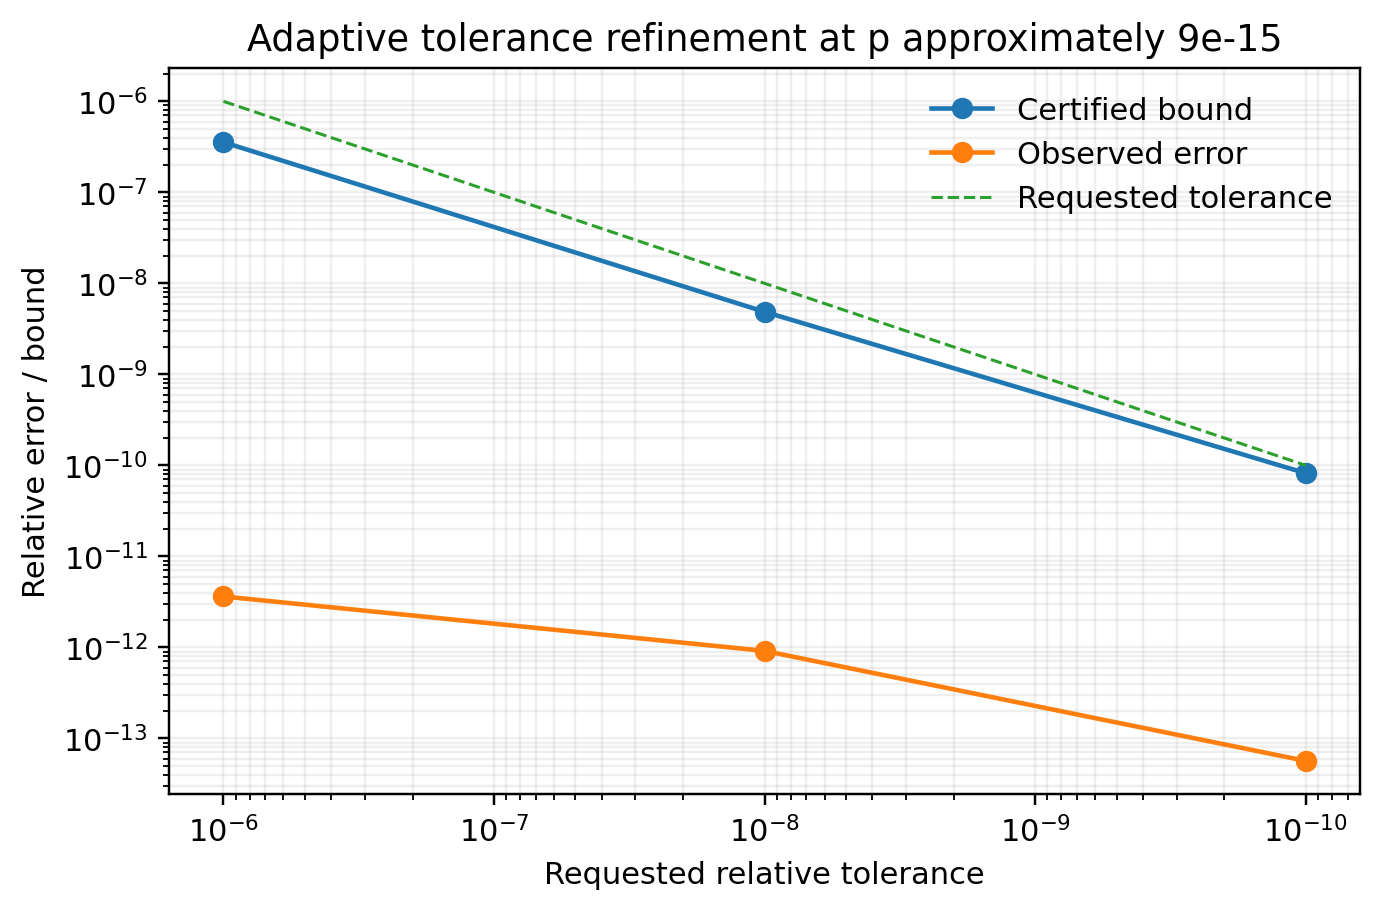
\includegraphics[width=0.78\linewidth]{figures/tolerance_ladder.png}
\caption{Requested tolerance, returned certificate, and observed error for one extreme-tail query.}
\label{fig:ladder}
\end{figure}

\subsection{Prototype runtime scaling}

Table \ref{tab:runtime} reports median CPU timings from the Python prototype. ``Adaptive total'' includes planning and certification. ``Compiled evaluation'' measures reuse of an already compiled spectral passport at the selected grid.

\begin{table}[htbp]
\centering
\caption{Prototype runtime scaling on genotype-derived spectra.}
\label{tab:runtime}
\begin{tabular}{rrrrrr}
\toprule
Rank & Packets & Exact tilted & Adaptive total & Compiled eval. & Compiled speedup\\
\midrule
397  & 13 & 6.66 ms & 10.45 ms & 0.549 ms & $12.1\times$\\
797  & 16 & 13.32 ms & 11.49 ms & 0.604 ms & $22.0\times$\\
1197 & 17 & 21.52 ms & 11.24 ms & 0.651 ms & $33.1\times$\\
\bottomrule
\end{tabular}
\end{table}

\begin{figure}[htbp]
\centering
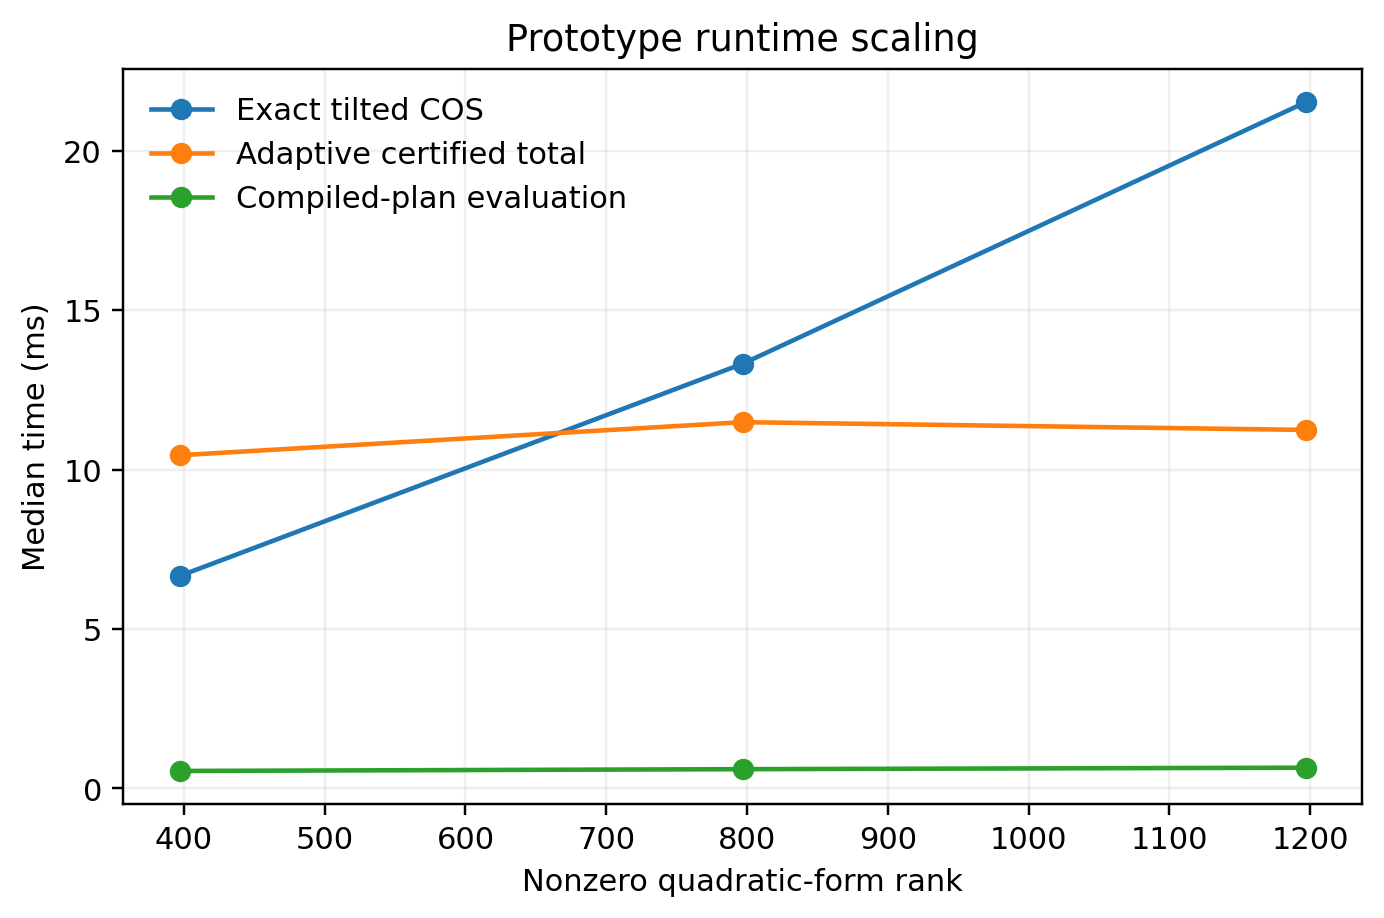
\includegraphics[width=0.78\linewidth]{figures/runtime_scaling.png}
\caption{Median runtime of exact tilted COS, adaptive certified K-COS including planning, and evaluation of an already compiled passport.}
\label{fig:runtime}
\end{figure}

The planning overhead matters. At rank 397, one certified adaptive query is slower than one exact tilted-COS query. The crossover appears between ranks 397 and 797 in this prototype, while compiled reuse is much faster. No universal speedup claim is therefore made.

\section{Relation to prior work and novelty boundary}

The mathematical ingredients surrounding K-COS overlap substantially with established literature:
\begin{itemize}
\item Imhof and Davies developed characteristic-function inversion methods for quadratic forms and linear combinations of chi-square variables \cite{Imhof1961,Davies1980}.
\item Saddlepoint approximations for quadratic forms are classical; see, for example, Kuonen \cite{Kuonen1999}.
\item The COS method and its characteristic-function coefficients are due to Fang and Oosterlee \cite{FangOosterlee2008}.
\item Rigorous COS parameter selection and convergence analysis have been developed in later work \cite{Junike2024,JunikeStier2025}.
\item Modern generalized-chi-square software includes additional exact and approximate algorithms, including recent ray-tracing, inverse-FFT, ellipse, and tail methods \cite{Das2025}.
\end{itemize}

Accordingly, this manuscript does \emph{not} claim novelty for exponential tilting, damping, saddlepoint centering, COS inversion, or the general idea of selecting Fourier truncation parameters from error bounds.

The candidate contribution is the specific representation layer between the spectrum and the transform:
\begin{enumerate}[label=(\alph*)]
\item centered local moment packets for the generalized-chi-square CGF rather than a global moment-matched surrogate distribution;
\item packet refinement driven by the actual complex tilted-COS query grid;
\item explicit propagation of packet log-CGF remainder into the tail functional;
\item joint error-budget refinement across spectral representation, support/periodization, and COS-mode truncation;
\item a reusable query-specific ``spectral passport'' whose post-compilation transform cost depends on packet count rather than raw rank.
\end{enumerate}

A literature search performed for this note did not identify this exact construction, but that is not a proof of priority. In particular, spectral aggregation, rational approximation, model reduction, and specialized weighted-chi-square literatures require a deeper audit before a formal novelty claim should be made.

\section{Limitations and next validation steps}

Several boundaries are material.

\paragraph{No Davies or Imhof benchmark yet.}
The current experiments compare against exact chi-square values, high-resolution exact-spectrum tilted COS, and in the development code, independent exponential-tilt importance sampling. They do not yet compare directly against Davies' algorithm or Imhof inversion. Such a benchmark is necessary for an external accuracy and speed claim.

\paragraph{Positive central quadratic forms only.}
The formal results above assume $\lambda_j>0$ and central $Z_j^2$ components. Indefinite forms, noncentral chi-square components, and additional Gaussian linear terms require extensions of both the transform domain and support analysis.

\paragraph{Analytic, not machine-verified, certification.}
The certificate bounds mathematical approximation error but not the rounding error of the numerical library. Directed-rounding interval arithmetic would be needed for a formally enclosed floating-point result.

\paragraph{Synthetic genotype benchmark.}
The SKAT-like experiments use genotype-derived synthetic spectra. Production validation should include real kernel spectra, larger ranks, null-model variants, and the same inputs passed to established SKAT/Davies implementations.

\paragraph{Planner optimality.}
Proposition \ref{prop:finite-refinement} establishes finite representability, not optimality of the current greedy planner. Better budget allocation may reduce compilation time or packet count.

\section{Conclusion}

K-COS treats a weighted chi-square spectrum not as a fixed list that must be revisited at every Fourier frequency, but as a query-dependent object that can be compressed, refined, and certified. The central formal mechanism is the centered packet expansion \eqref{eq:packet-expansion} with the local remainder \eqref{eq:packet-remainder}. Exponential tilting places an extreme-tail query near the center of the transformed law, positivity removes lower-support truncation, and the explicit tilted characteristic-function modulus yields a direct omitted-mode bound. Together these produce the combined certificate \eqref{eq:combined}.

The current results support further development, but they do not yet establish superiority over mature generalized-chi-square algorithms. The next decisive experiment is a common-input benchmark against Davies, Imhof, and modern generalized-chi-square methods over central, extreme-tail, high-rank, spiked, and nearly rank-deficient spectra. If the measured speed and accuracy advantages survive that comparison, the centered spectral compiler would constitute the main numerical contribution.

\appendix
\section{Closed-form quantities used by the implementation}

The saddlepoint derivatives follow from \eqref{eq:derivatives}. Under the tilt, the variance and fourth cumulant are
\[
\kappa''(\theta)
=2\sum_j\frac{\lambda_j^2}{(1-2\theta\lambda_j)^2},
\]
\[
\kappa^{(4)}(\theta)
=48\sum_j\frac{\lambda_j^4}{(1-2\theta\lambda_j)^4}.
\]
The prototype initializes the upper support as
\[
b=q+L\sqrt{\kappa''(\theta_*)+\sqrt{\kappa^{(4)}(\theta_*)}},
\]
then lets the support certificate determine whether $L$ must grow. This initialization is a heuristic scale choice; the returned certificate, rather than the formula itself, determines acceptance.

For the tilted Chernoff step, the optimizing parameter $\eta$ solves $\kappa'(\eta)=b$. Because $b>q=\kappa'(\theta_*)$ and $\kappa'$ is strictly increasing, the optimizer is unique in $(\theta_*,1/(2\lambda_{\max}))$.

\section{Reproducibility record}

The prototype used for the reported Block 3 experiments returned the following summary:
\begin{itemize}
\item regression tests: 3/3 passed;
\item requested analytic tolerance in the twelve-spectrum suite: $10^{-8}$;
\item worst observed relative error: $6.148608\times10^{-11}$;
\item largest certified relative bound: $7.917203\times10^{-9}$;
\item rank-scaling experiment: 397, 797, 1197;
\item compiled-plan evaluation speedups relative to exact tilted COS at the same selected $N,L$: $12.1\times$, $22.0\times$, $33.1\times$.
\end{itemize}
The code package associated with this draft is \texttt{KCOS\_Block3\_AdaptiveCertified\_2026-09-23}.

\begin{thebibliography}{99}

\bibitem{Davies1980}
R. B. Davies,
``The distribution of a linear combination of chi-squared random variables,''
\emph{Applied Statistics}, vol. 29, pp. 323--333, 1980.

\bibitem{Das2025}
A. Das,
``New methods to compute the generalized chi-square distribution,''
\emph{Journal of Statistical Computation and Simulation}, vol. 95, no. 12, pp. 2608--2642, 2025.
DOI: \href{https://doi.org/10.1080/00949655.2025.2501401}{10.1080/00949655.2025.2501401}.

\bibitem{FangOosterlee2008}
F. Fang and C. W. Oosterlee,
``A novel pricing method for European options based on Fourier-cosine series expansions,''
\emph{SIAM Journal on Scientific Computing}, vol. 31, no. 2, pp. 826--848, 2008.
DOI: \href{https://doi.org/10.1137/080718061}{10.1137/080718061}.

\bibitem{Imhof1961}
J. P. Imhof,
``Computing the distribution of quadratic forms in normal variables,''
\emph{Biometrika}, vol. 48, nos. 3--4, pp. 419--426, 1961.
DOI: \href{https://doi.org/10.1093/biomet/48.3-4.419}{10.1093/biomet/48.3-4.419}.

\bibitem{Junike2024}
G. Junike,
``On the number of terms in the COS method for European option pricing,''
\emph{Numerische Mathematik}, vol. 156, pp. 533--564, 2024.
DOI: \href{https://doi.org/10.1007/s00211-024-01402-1}{10.1007/s00211-024-01402-1}.

\bibitem{JunikeStier2025}
G. Junike and H. Stier,
``From characteristic functions to multivariate distribution functions and European option prices by the (damped) COS method,''
\emph{SIAM Journal on Numerical Analysis}, vol. 63, no. 6, pp. 2421--2453, 2025.
DOI: \href{https://doi.org/10.1137/24M1666240}{10.1137/24M1666240}.

\bibitem{Kuonen1999}
D. Kuonen,
``Saddlepoint approximations for distributions of quadratic forms in normal variables,''
\emph{Biometrika}, vol. 86, no. 4, pp. 929--935, 1999.

\bibitem{Liu2009}
H. Liu, Y. Tang, and H. H. Zhang,
``A new chi-square approximation to the distribution of non-negative definite quadratic forms in non-central normal variables,''
\emph{Computational Statistics \& Data Analysis}, vol. 53, pp. 853--856, 2009.

\bibitem{Wu2011}
M. C. Wu, S. Lee, T. Cai, Y. Li, M. Boehnke, and X. Lin,
``Rare-variant association testing for sequencing data with the sequence kernel association test,''
\emph{American Journal of Human Genetics}, vol. 89, no. 1, pp. 82--93, 2011.
DOI: \href{https://doi.org/10.1016/j.ajhg.2011.05.029}{10.1016/j.ajhg.2011.05.029}.

\end{thebibliography}

\end{document}
